\section{Tuesday, 27 November 2018}

\subsection{Steps}
\begin{itemize}
\item We tried to merge the dataset with \texttt{merge\_asof} but we had the problem that the data didn't associate the correct form.

After that, we applied \textit{Naive Bayer} to make the prediction and see the results with that prediction. In simple terms, a Naive Bayes classifier assumes that the presence of a particular feature in a class is unrelated to the presence of any other feature. For example, a fruit may be considered to be an apple if it is red, round, and about 3 inches in diameter. Even if these features depend on each other or upon the existence of the other features, all of these properties independently contribute to the probability that this fruit is an apple and that is why it is known as ‘Naive’.

\begin{figure}[H]
	\begin{center}
		

	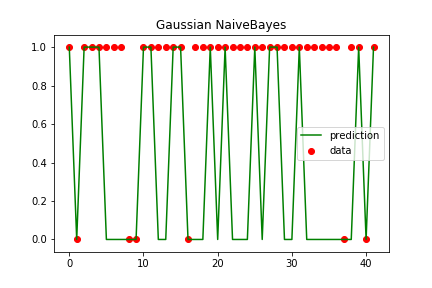
\includegraphics[width=0.7\linewidth]{../../reports/figures/NaiveBayesPrediction}
	\label{fig:naivebayesprediction}
		\end{center}
\end{figure}

The line represents the prediction of Naive Bayes and the points the real data. When the point coincides with the line, the algorithm is successful, otherwise it is considered a failure

\item Classification is computed from a simple majority vote of the nearest neighbors of each point: a query point is assigned the data class which has the most representatives within the nearest neighbors of the point.

\begin{figure}[H]
	\begin{center}
	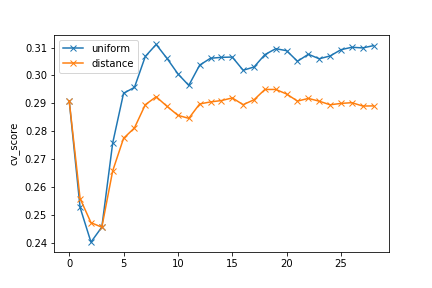
\includegraphics[width=0.7\linewidth]{../../reports/figures/KNearestNeighborsAlgorithm}
	\label{fig:knearestneighborsalgorithm}
	\end{center}
\end{figure}
\begin{itemize}
	\item \textbf{Uniform weights}: each point in the local neighborhood contributes uniformly to the regression of a query point.
	\item \textbf{Distance weights}: weight points such that nearby points contribute more to the regression than faraway points.
\end{itemize}
	The intersection of the two measures gives us the optimum number of neighbors.
	
	\item From the optimal number of neighbors we did the regression.
\begin{figure}[H]
	\begin{center}
	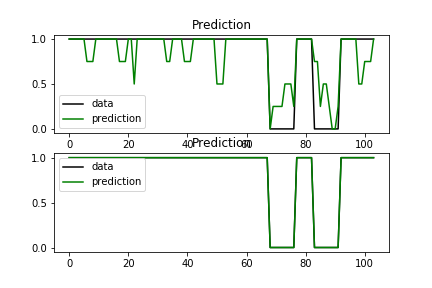
\includegraphics[width=0.7\linewidth]{../../reports/figures/Prediction}
	\label{fig:prediction}
	\end{center}
\end{figure}
	
\end{itemize}
